\documentclass[xcolor=dvipsnames]{beamer}

% ==== 主題 ====
\usetheme{metropolis}
\usefonttheme{professionalfonts}          % 不覆蓋你自訂的字型

% ==== 字型 ====
\usepackage{fontspec}
\usepackage{xeCJK}
\renewcommand{\familydefault}{\rmdefault} % 使用 serif 字體（重點）

% 西文字型：Times New Roman 的開源替代品
\setmainfont{TeX Gyre Termes}[
  Ligatures=TeX,
  BoldFont={* Bold},
  ItalicFont={* Italic}
]

% 中文字型（可改為思源宋體、標楷體等）
\setCJKmainfont{Noto Serif CJK TC}
\setCJKsansfont{Noto Sans CJK TC} % 有需要再用
\setCJKmonofont{Noto Sans Mono CJK TC}

% ==== 數學字型（與正文字體一致）====
\usepackage{unicode-math}
\setmathfont{TeX Gyre Termes Math}

% ==== 套件 ====
\usepackage{amsmath, amssymb}
\usepackage{graphicx}
\usepackage{hyperref}
\usepackage{minted}
\usepackage{fvextra}
\usepackage{xcolor}
\usepackage{booktabs}
\usepackage{tabularx}
\usepackage{multicol}

% ==== 顏色設定（可選）====
\definecolor{MyBlue}{RGB}{3, 55, 105}
\setbeamercolor{structure}{fg=MyBlue}
\setbeamercolor{block title}{bg=MyBlue,fg=white}
\setbeamercolor{block body}{bg=blue!5}
\setbeamertemplate{section in toc}{%
  \inserttocsectionnumber.~\inserttocsection\par
}

\setminted{
    linenos,                % 行號
    frame=lines,            % 上下框線
    framesep=5pt,           % 程式碼與邊框距離
    numbersep=8pt,          % 行號與程式碼距離
    fontsize=\scriptsize,   % 字體大小
    breaklines,             % 自動換行
    tabsize=4,              % tab 寬度
    rulecolor=\color{black},% 框線顏色
    xleftmargin=1.5em       % 左側縮排
}

\title{以建置數位孿生系統爲目標，如何整合建物生產履歷資料及成爲未來客戶運維及資產管理系統。}
\author{Tai, Wei Hsuan}
\date{SGS 引路人實習面試}

\begin{document}
	\begin{frame}
		\titlepage
	\end{frame}

    \begin{frame}
        \frametitle{Outline}
        \tableofcontents
    \end{frame}
    \section{Introduction}
    \begin{frame}
        \begin{figure}
            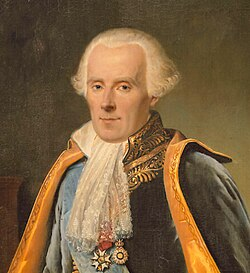
\includegraphics[width=0.8\textwidth]{src/Pierre-Simon_Laplace.jpg}
        \end{figure}
    \end{frame}
    \begin{frame}
        \frametitle{什麼是數位孿生？}
        \begin{itemize}
            \item 將現實世界的物理實體在數位空間中創建一個虛擬模型。
            \item 通常結合 IoT、AI、Big Data 等技術。
            \item 實時反映物理實體的狀態、行為和性能。
        \end{itemize}
    \end{frame}
    \begin{frame}
        \frametitle{Unmet Needs}
        考慮以下幾種情境：
        \begin{enumerate}
            \item 發生重大事故（如：火災）
            \item 業主想要裝潢
            \item 設備老舊
        \end{enumerate}
        解法多為「參考圖紙」、「技師現場勘查」，但圖紙不一定準確，技師也不一定能夠完全掌握建物的狀況。
    \end{frame}

    \section{Implementation}
    \begin{frame}
        \frametitle{要儲存的資料}
        \begin{enumerate}
            \item 硬體資料
            \item 履歷資料
            \item 操作資料
        \end{enumerate}
    \end{frame}
    \begin{frame}
        \frametitle{硬體資料}
        \begin{itemize}
            \item 零組件的外觀規格（如：尺寸、重量），直接透過圖紙取得
            \item 零組件的內部結構（如：材料、細微內部結構），可透過X-ray、超音波等非破壞性檢測技術取得
            \item 建物的內部結構（已經建造完成的），透過3D掃描、超音波等非破壞性檢測技術取得
        \end{itemize}
    \end{frame}
    \begin{frame}
        \frametitle{履歷資料}
        \begin{itemize}
            \item 零組件的生產履歷（如：產線、生產日期、製造商）
            \item 零組件的運輸履歷（如：運輸方式、運輸時間、運輸路線）
            \item 零組件的儲存履歷（如：儲存環境、儲存時間）
        \end{itemize}
    \end{frame}
    \begin{frame}
        \frametitle{操作資料}
        \begin{itemize}
            \item 施工時的操作資料（如：施工人員、施工時間、施工方法）
            \item 使用時的操作資料（如：使用者、使用時間、使用頻率）
            \item 使用時的環境資料（如：溫度、濕度、震動）
        \end{itemize}
    \end{frame}
    \begin{frame}
        \frametitle{資料的儲存}
        \begin{itemize}
            \item 利用一個RDBMS儲存資料，每個零件有其唯一的UUID
            \item 零組件組成建物，建物也有其唯一的UUID，並且可以追蹤每個零組件的UUID，再由零組件的UUID追蹤到零組件的資料
        \end{itemize}
        
    \end{frame}
    \begin{frame}
        \frametitle{資料的使用方法}
        \begin{itemize}
            \item 查詢現況（這個零組件的結構長怎樣）
            \item 即時監控（哪邊有異常）
            \item 即時預警（這棟建物哪邊的結構可能疲勞老化）
            \item 建議查詢（給予裝潢時的建議）
        \end{itemize}
    \end{frame}
    \begin{frame}
        \frametitle{雙向數位孿生}
        \begin{enumerate}
            \item 根據實體狀況建立數位模型以模擬
            \item 在數位模型完成模擬後再根據規格生產實體
        \end{enumerate}
    \end{frame}

    \section{Examples}
    \begin{frame}
        \frametitle{案例1：火災}
        \begin{itemize}
            \item 設計時考慮火災的情境，最佳化建物的內部結構
            \item 平時在虛擬環境模擬火災，給出最佳逃生路線
            \item 發生火災，直接給予消防隊建物內部結構圖
            \item 發生火災，現場分析建物內部結構，給出倒塌風險
        \end{itemize}
    \end{frame}
    \begin{frame}
        \frametitle{案例2：裝潢}
        \begin{itemize}
            \item 提供設計師現有模型，方便設計師在此基礎上進行裝潢設計
            \item 模擬裝潢後的建物狀況，分析可能的安全隱患
            \item 模擬裝潢後的建物狀況，分析對舒適度的影響
        \end{itemize}
    \end{frame}
    \begin{frame}
        \frametitle{案例3:預測性維修}
        \begin{itemize}
            \item 利用IoT感測器收集建物的使用資料，分析建物的狀況
            \item 某電梯使用頻率極高，提前預警老化
            \item 某空調系統長期超載，提前預警老化
        \end{itemize}
    \end{frame}


    \section{Conclusion}

    \begin{frame}{數位孿生的好處}
        對公司的好處
        \begin{itemize}
            \item 維持口碑、競爭力
            \item 長期綁定客戶
        \end{itemize}
        對客戶的好處
        \begin{itemize}
            \item 提高安全性
            \item 提高舒適度
            \item 降低維修成本
        \end{itemize}
    \end{frame}
    \begin{frame}
        \frametitle{如何降低成本}
        \begin{itemize}
            \item 定期模擬老化狀況，非時時模擬
            \item 紀錄零組件內部結構時紀錄「最低強度」，非紀錄完整結構
            \item 優先保存重要零組件的資料，非全部零組件
        \end{itemize}
    \end{frame}
    \begin{frame}
        \frametitle{數位孿生可能引發的問題}
        \begin{itemize}
            \item 資料隱私和安全問題
            \item 技術整合的挑戰
            \item 成本和資源的投入
        \end{itemize}
    \end{frame}
\end{document}